% ---------------------------------------------------------------------------- %
\section{Software \Master}
\label{sec:software:master}
% ---------------------------------------------------------------------------- %

Im   Folgenden  werden   die  verwendeten   Komponenten  der   Master-Software
beschrieben   und    es   wird    auf   die   Lizenzen    dieser   Komponenten
eingegangen. Anschliessend werden  der Aufbau unseres Software-Stacks  und die
Funktionsprinzipien dokumentiert.


% ---------------------------------------------------------------------------- %
\subsection{Komponenten}
\label{subsec:software:master:components}
% ---------------------------------------------------------------------------- %

Als Betriebssystem kommt Raspbian zum  Einsatz. Raspbian ist eine Variante von
Debian-Linux mit  einigen Erweiterungen, welche  das System auf  einem \Raspi~
lauff\"ahig machen. Als  graphische Oberfl\"ache wird LXDE  benutzt, aufbauend
auf  X11. Die wichtigsten  Komponenten des  Software-Stacks sind  in Abbildung
\ref{fig:softwarestack} dargestellt.

Die  Funktionalit\"at  unserer  Software  wird  mit  einigen  Python-Libraries
implementiert. PyQt wird  benutzt, um  die graphische  Benutzeroberfl\"ache zu
programmieren, SQLAlchemy  dient als  Datenbanktreiber und  \emph{WiringPi for
Python} ist  daf\"ur verantwortlich,  die Hardware-Schnittstellen  des \Raspi~
zu  abstrahieren und  in Python  bereitzustellen. Tabelle \ref{tab:pythonLibs}
listet die Libraries und ihre Aufgaben in einer \"Ubersicht auf.

\begin{figure}[h!tb]
    \centering
    \begin{bytefield}{32}
        %\begin{rightwordgroup}{Adresse}
        \colorbitbox{solarized-base2}  {solarized-base02}{32}{Unsere Software} \\
        \colorbitbox{solarized-blue}   {solarized-base3}  {8}{PyQt}
        \colorbitbox{solarized-blue}   {solarized-base3}  {8}{SQLAlchemy}
        \colorbitbox{solarized-blue}   {solarized-base3}  {8}{WiringPi}
        \colorbitbox{solarized-magenta}{solarized-base3}  {8}{LXDE} \\
        \colorbitbox{solarized-blue}   {solarized-base3} {24}{Python 3}
        \colorbitbox{solarized-magenta}{solarized-base3}  {8}{X11} \\
        \colorbitbox{solarized-base01} {solarized-base3} {32}{Linux} \\
        %\end{rightwordgroup} \\
  \end{bytefield}
  \caption{Software-Stack f\"ur unser Projekt}
  \label{fig:softwarestack}
\end{figure}

\begin{table}[h!tb]
    \centering
    \caption{Liste der verwendeten Python-Libraries}
    \label{tab:pythonLibs}
    \small
    \begin{tabular}{lrp{50mm}r}
        \toprule
        \textsc{Library} & \textsc{Version} & \textsc{Zweck} & \textsc{Website} \\
        \midrule
        PyQt & 5 & Erstellen und verwalten der graphischen Bedienelemente & \cite{ref:pyqt} \\
        [5mm]
        \rowcolor{solarized-base2}
        SQLAlchemy & 1.0 & Datenbankabstraktion                           & \cite{ref:sqlalchemy} \\
        [5mm]
        WiringPi for Python & 2 & Abstraktion der Hardware-Schnittstellen & \cite{ref:wiringpi} \\
        \bottomrule
    \end{tabular}
\end{table}

% ---------------------------------------------------------------------------- %
\clearpage
\subsection{Lizenzen}
\label{subsec:software:master:licenses}
% ---------------------------------------------------------------------------- %

Bei    der   Auswahl    von    Drittsoftware   wird    auf   die    jeweiligen
Lizenzbedingungen   geachtet,   um   keine   Konflikte   zu   verursachen. Die
wichtigsten  drei Lizenz-Bereiche  und ihre  Charakteristiken sind  in Tabelle
\ref{tab:licenseAreas} aufgef\"uhrt.

\begin{table}[h!tb]
    \centering
    \caption{Lizenzbereiche}
    \label{tab:licenseAreas}
    \small
    \begin{tabular}{>{\raggedright}p{30mm}>{\raggedright}p{30mm}p{50mm}}
        \toprule
        \textsc{Bereich} &
        \textsc{Lizenz} &
        \textsc{Bedingungen} \\
        \midrule
        Linux-Kernel &
        GPL &
        Quellcode und \"Anderungen m\"ussen \"offentlich sein. \\
        [3mm]

        \rowcolor{solarized-base2}
        Treiber f\"ur Raspberry Pi und Display &
        Restricted &
        Quellcode wird vom Hersteller geheim gehalten \\
        [8mm]

        Raspbian &
        DFSG (Sammlung diverser Lizenzen) &
        Darf frei verwendet, aber nicht unbedingt verkauft, werden. \\
        \bottomrule
    \end{tabular}
\end{table}

Grundlage  f\"ur die  Software  bildet  das angepasste  Betriebssystem. Dieses
wird  von  der Raspberry  Pi  Foundation  frei  zur Verf\"ugung  gestellt  und
unterliegt den  Bedingungen den  DFSG (\emph{Debian Free  Software Guidelines}
\cite{ref:socialContract}). Die  darauf  aufbauenden Programmbibliotheken  zur
Abstraktion  von Betriebsystemfunktionen  und weiteren  Hardware-Aufrufen sind
alle aus den Raspbian-Repositories verf\"ugbar und unterliegen daher ebenfalls
den  DFSG.   Da  die  Mastersoftware zwar  auf  diesen  Komponenten  aufsetzt,
sie  aber  nicht ver\"andert  oder  statisch  verlinkt wird,  entstehen  keine
Lizenzkonflikte. Zu beachten ist hier, dass diese Drittsoftware im Allgemeinen
nicht als Eigenwerk  verkauft werden darf. Das heisst, dass  sie zwar beliebig
verbreitet werden darf, nicht aber zum Produkt hinzugez\"ahlt werden kann.

Die DFSG stellen  insbesondere folgende Anforderung an  alle Programme, welche
Teil von Raspbian sind:

\begin{itemize}
    \tightlist
\item
    Die Software darf frei verbreitet werden (Regel 1)
\item
    Die Software darf f\"ur beliebige Zwecke eingesetzt werden (Regel 6)
\item
    Die Software beschr\"ankt unzusammenh\"angende Software nicht (Regel 9)
\end{itemize}

Der eigentliche  Mastersoftware-Quellcode dagegen  ist nicht  \"offentlich und
kann als Bestandteil des Produkts verkauft werden.



% ---------------------------------------------------------------------------- %
\subsection{Threads}
\label{subsec:software:master:threads}
% ---------------------------------------------------------------------------- %


Die  Mastersoftware  ist in  mehrere  Threads  gegliedert, unter  welchen  die
Funktionen aufgeteilt  sind. Sie werden alle von  einem Hauptthread gestartet,
welcher die Koordination mittels Semaphoren \"ubernimmt. Dazu initialisiert er
alle  Resourcen,  auf  welche  aus  mehreren  Threads  zugegriffen  sind. Dies
sind  Datenbank und  Logging-System, welche  beide Multithreading  beherrschen
und  threadsafe  sind. Die zentrale  Koordination  bedeutet  zudem, dass  alle
Arbeitsschritte nur sofern n\"otig und nicht mit veralteten Daten ausgef\"uhrt
werden.

Um  die Threadsicherheit  zu  gew\"ahrleisten, verwenden  die beiden  geteilten
Resourcen spezielle Mechanismen:
\begin{itemize}
    \tightlist
    \item
        Die   Loggingfunktion  setzt   eine   Queue  ein,   um  Meldungen   zu
        zwischenzuspeichern und asynchron hintereinander abzuarbeiten.
     \item
        SQLAlchemy beinhaltet  mit der  \emph{ScopedSession} eine  Methode, um
        aus  mehreren  Threads  parallel  aufgerufen  zu  werden. Dazu  werden
        die  Anfragen  aus jeweils  einem  Thread  gruppiert und  dann  atomar
        ausgef\"uhrt.
 \end{itemize}

Alle anderen externen Ressourcen (\ISC-bus,  UART und GPIO) werden jeweils von
nur einem Thread genutzt, wodurch keine Konflikte auftreten k\"onnen.

Im Detail sieht die Aufgabenteilung folgendermassen aus:
\begin{itemize}
    \tightlist
    \item
        \textbf{Prozesssteuerung:} Der  Hauptthread  verwaltet  Resourcen  und
        alle weiteren Threads.
    \item
        \textbf{Datensammlung:} Ein  Thread  empf\"angt   die  Spannungs-  und
        Strommesswerte von den Sensoren und speichert sie in der Datenbank ab.
    \item
        \textbf{Datenauswertung:} Ein   separater    Thread   untersucht   die
        gespeicherten  Messwerte   auf  defekte   Panels  und   speichert  die
        Ergebnisse ebenfalls in der Datenbank ab.
    \item
        \textbf{Graphisches  Benutzerinterface:} Der   GUI-Thread  stellt  ein
        Fenster  dar,   mit  welchem   der  Benutzer  die   Einstellungen  von
        Alarmierung  und   Telefonnummer  konfigurieren  kann   und  speichert
        \"Anderungen in der Datenbank.
    \item
        \textbf{Ausgabe:} Die  Umsetzung  der definierten  Massnahmen  obliegt
        einem Thread, welcher das Modem verwaltet und bei Bedarf die digitalen
        Ausg\"ange zur Steuerung der Relais bet\"atigt
\end{itemize}


% ---------------------------------------------------------------------------- %
\subsection{Benutzeroberfl\"ache}
\label{subsec:software:master:GUI}
% ---------------------------------------------------------------------------- %


Die Benutzeroberfl\"ache  ist in  PyQt5 implementiert. PyQt5 basiert  auf Qt5,
welches eine sehr verbreitete Library f\"ur GUI-Oberfl\"achen ist. Dadurch ist
sie extrem  feature-reich und  bringt alles  mit was  die Benutzeroberfl\"ache
braucht.

In  Qt5  gibt  es  das  sogenante  \code{MainWindow},  welches  alle  weiteren
Code-Teile unter sich b\"undelt. So werden  zum Beispiel auch separate Threads
wie die Schnittstelle zur UART dar\"uber gesteuert.

Das  GUI  besteht aus  mehreren  Views  in  Form vom  \code{QWidgets},  welche
mit   einem   \code{QStackedWidget}   gruppiert  und   angezeigt   werden. Das
\code{QStackedWidget}  erlaubt  es,  in  einem  bestimmten  Viewport  zwischen
verschiedenen \code{QWidgets} und somit verschiedenen Ansichten zu wechseln.

Um einen Fehler anzuzeigen, wird die \code{ErrorView} im \code{QStackedWidget}
selektiet. Zudem werden  die Parameter zum fehlerhaften  Modul \"ubergeben und
angezeigt.

\"Uber  Callbacks  k\"onnen  Prozesse  ausserhalb  des  GUIs  angestossen  und
kontrolliert werden.

\clearpage
\begin{wrapfigure}{r}{0.475\textwidth}
    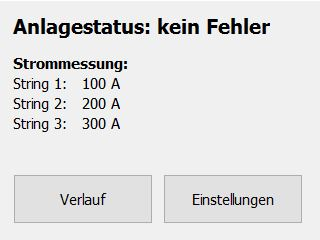
\includegraphics[width=0.475\textwidth]{images/userguide/screen0.jpg}
    \caption{Hauptmenu}
    \label{fig:software:gui:screen0}
\end{wrapfigure}

Die Benutzeroberfl\"ache  ist bewusst sehr schlicht  gehalten. Sie besteht aus
folgenden Ansichten: Hauptmen\"u, Einstellungen, Eingabe der Telefonnummer und
dem Fehlerverlauf,  gezeigt in den  Abbildungej \ref{fig:software:gui:screen0}
bis     \ref{fig:software:gui:screen4}. Die     Beschreibung    der     vollen
Funktionalit\"at  ist  im  Kapitel \emph{\titleref{chap:userguide}}  ab  Seite
\pageref{chap:userguide} zu finden.

\vspace*{6em}
\noindent\adjustbox{valign=t}{\begin{minipage}{0.475\textwidth}
    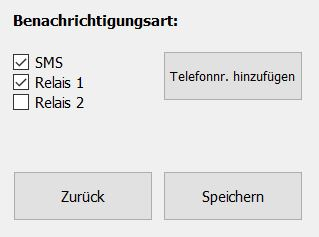
\includegraphics[width=\textwidth]{images/userguide/screen1.jpg}
    \figcaption[Master: Menu: Einstellungen]{Einstellungen}
    \label{fig:software:gui:screen1}
\end{minipage}}
\hspace*{0.04\textwidth}
\noindent\adjustbox{valign=t}{\begin{minipage}{0.475\textwidth}
    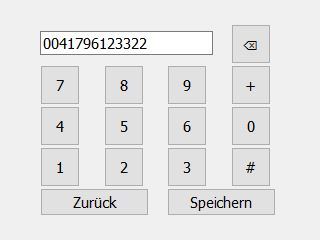
\includegraphics[width=\textwidth]{images/userguide/screen2.jpg}
    \figcaption[Master: Menu: Einstellungen: Telefonnummer]{Eingabe einer Telefonnummer}
    \label{fig:software:gui:screen2}
\end{minipage}}

\noindent\adjustbox{valign=t}{\begin{minipage}{0.475\textwidth}
    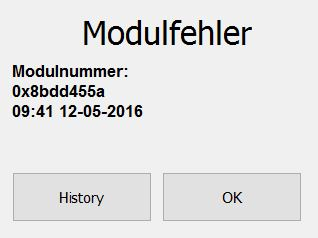
\includegraphics[width=\textwidth]{images/userguide/screen3.png}
    \figcaption[Master: Menu: Modulfehler]{Fehler bei einem Modul}
    \label{fig:software:gui:screen3}
\end{minipage}}
\hspace*{0.04\textwidth}
\noindent\adjustbox{valign=t}{\begin{minipage}{0.475\textwidth}
    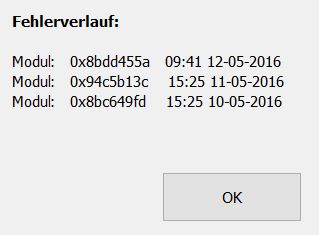
\includegraphics[width=\textwidth]{images/userguide/screen4.jpg}
    \figcaption[Master: Menu: Einstellungen: Fehlerverlauf]{Fehlerverlauf der Anlage}
    \label{fig:software:gui:screen4}
\end{minipage}}

% ---------------------------------------------------------------------------- %
\clearpage
\subsection{Datenbank}
\label{subsec:software:master:database}
% ---------------------------------------------------------------------------- %


Um  die  gesammelten  Daten  optimal  zu speichern  und  zu  einem  sp\"ateren
Zeitpunkt wieder  verwenden zu  k\"onnen, wird eine  Datenbank verwendet. Dies
hat gegen\"uber  der Verwendung von internen  Datenstrukturen wie Dictionaries
und Arrays  zwar die Nachteile von  gr\"osserem (Erst-)Implementationsaufwand,
h\"oherem  Arbeitsspeicherbedarf  und   gr\"osserem  Rechenaufwand  f\"ur  die
CPU. Jedoch   wird  die   Wartung  der   Software  und   das  Erg\"anzen   von
zus\"atzlicher   Funktionalit\"at   stark   vereinfacht. Ebenfalls   ist   die
Auswertung einfacher und  flexibler, da schon beim Auslesen der  Werte aus der
Datenbank nach verschiedenen Kriterien gefiltert werden kann.

\begin{figure}[h!tb]
    \centering
    \begin{tikzpicture}
    \sffamily
    \small
    %\graph [left anchor=east,grow right sep,right anchor=west,grow right,branch down,nodes={rounded rectangle,draw}]
    \begin{scope}[
            every node/.style = {
                draw = solarized-base02,
                rounded rectangle,
                fill=solarized-base2,
                text=solarized-base02,
                inner sep=1mm,
                text height=0.7em,
            },
            node distance=3mm,
            table/.style={
                fill=solarized-cyan,
                text=solarized-base2,
                inner sep=2mm,
            },
            column/.style={
                minimum width=25mm,
            }
        ]
        \node (database)[
            fill=solarized-blue,
            text=solarized-base2,
            inner sep=2mm
        ] at (0,0) {Datenbank};

        \node (strings)   [table,below left=15mm of database] {strings};
        \node (sID)       [column,below right=12mm of strings] {ID};
        \node (sStringNo) [column,below=of sID]            {stringnumber};
        \node (sCurr)     [column,below=of sStringNo]      {stringcurrent};
        \node (sTs)       [column,below=of sCurr]          {timestamp};
        \node (sDev)      [column,below=of sTs]            {deviation};
        \node (sReported) [column,below=of sDev]           {flag\_reported};

        \node (panels)    [table,left=of strings]  {panels};
        \node (pID)       [column,below left=12mm of panels]    {ID};
        \node (pSerial)   [column,below=of pID]       {serialnumber};
        \node (pVoltage)  [column,below=of pSerial]   {voltage};
        \node (pStringNo) [column,below=of pVoltage]  {stringnumber};
        \node (pTs)       [column,below=of pStringNo] {timestamp};
        \node (pDev)      [column,below=of pTs]       {deviation};
        \node (pReported) [column,below=of pDev]      {flag\_reported};

        \node (string1)  [table,below right=15mm of database] {string\{1,2,3\}};
        \node (s1ID)     [column,below right=12mm of string1]        {ID};
        \node (s1Serial) [column,below=of s1ID]           {serialnumber};
    \end{scope}
    \begin{scope}[on background layer]
    \end{scope}

    \begin{scope}[
            rounded corners,
            draw=solarized-base02
        ] % connections
        \draw[-latex] (database) -| (panels);
        \draw[-latex] (database) -| (strings);
        \draw[-latex] (database) -| (string1);

        \draw[-latex] (panels) |- (pID);
        \draw[-latex] (panels) |- (pSerial);
        \draw[-latex] (panels) |-  (pVoltage);
        \draw[-latex] (panels) |-  (pStringNo);
        \draw[-latex] (panels) |-  (pTs);
        \draw[-latex] (panels) |-  (pDev);
        \draw[-latex] (panels) |-  (pReported);

        \draw[-latex] (strings) |- (sID);
        \draw[-latex] (strings) |- (sStringNo);
        \draw[-latex] (strings) |- (sCurr);
        \draw[-latex] (strings) |- (sTs);
        \draw[-latex] (strings) |- (sDev);
        \draw[-latex] (strings) |- (sReported);

        \draw[-latex] (string1) |- (s1ID);
        \draw[-latex] (string1) |- (s1Serial);
    \end{scope}
\end{tikzpicture}

    \caption{Datenbank-Layout}
  \label{fig:database:layout}
\end{figure}


%stringX-tables:
Unsere Datenbank  umfasst 5 Tabellen  (oder \emph{Tables} im  Fachjargon), wie
auch in Abbildung \ref{fig:database:layout} gezeigt:

\begin{itemize}
    \tightlist
    \item
        \code{panels:} Speichert die Spannungen der PV-Module
    \item
        \code{strings:} Speichert die Str\"ome in den Strings
    \item
        \code{string1:} Speichert Sensor-IDs in String 1
    \item
        \code{string2:} Speichert Sensor-IDs in String 2
    \item
        \code{string3:} Speichert Sensor-IDs in String 3
\end{itemize}

Letztere drei  (in Abbildung \ref{fig:database:layout} auf  der rechten Seite)
davon  dienen  ausschliesslich  der  Zuordnung  aller  im  System  vorhandenen
Seriennummern  zu  den  einzelnen  Strings. Dies ist  notwendig,  um  bei  der
Auswertung  zu wissen,  welche Sensoren  sich  im selben  String befinden  und
dementsprechend miteinander verglichen  werden m\"ussen. Diese Tables bestehen
lediglich aus 2  Spalten, eine f\"ur die Seriennummer sowie  eine f\"ur die ID
des  Eintrages, welcher  ben\"otigt wird,  um doppelt  eingetragene Zeilen  zu
verhindern.

%strings-table:
Das Table \code{strings} (Mitte  in Abbildung \ref{fig:database:layout}) dient
der Speicherung  der gemessenen String-Str\"ome. Diese Werte  werden als Paket
mit einigen  wichtigen zus\"atzlichen Daten gespeichert. Dazu  geh\"oren neben
dem gemessenen Stromwert noch die  String-Nummer, um zu wissen, welcher String
gemessen worden ist,  ein Zeitstempel, um nachvollziehen zu  k\"onnen, wie alt
die Eintr\"age  sind, ein leeres  Feld, um  bei der Auswertung  die Abweichung
zum  Durchschnitt eintragen  zu k\"onnen,  sowie  ein Feld,  welches ein  Flag
beinhaltet, das  anzeigt, ob  der String bereits  als ausserhalb  der Toleranz
gemeldet  worden  ist. Zudem wird  auch  hier  wieder  eine Spalte  f\"ur  die
Eintrags-ID ben\"otigt.

%panels-table:
Das  letzte  und  gr\"osste  Table   ist  \code{panels}  (links  in  Abbildung
\ref{fig:database:layout}),  in  welchem   die  Modulspannungen  abgespeichert
werden. Auch  hier   wird  dies   wieder  als   Paket  mit   relevanten  Daten
realisiert. Die  Zeile in  diesem Table  ist grunds\"atzlich  gleich aufgebaut
wie  jene des  Strings-Table, nur  dass  hier anstelle  des String-Stroms  die
Modulspannung eingetragen sowie ein zus\"atzliches Feld f\"ur die Seriennummer
des  gemessenen  Modul-Sensors  verwendet wird. Dies  wird  hier  zus\"atzlich
ben\"otigt,  um  die  gemessenen  Daten   in  direktem  Zusammenhang  mit  den
Seriennummern  der Sensoren  zu bringen,  was f\"ur  die Auswertung  der Daten
n\"otig ist.


% ---------------------------------------------------------------------------- %
\subsection{Implementation}
\label{subsec:software:master:implementation}
% ---------------------------------------------------------------------------- %

Die  Master-Software  besteht aus  Python-Files,  auf  welche die  anfallenden
Aufgaben  verteilt  werden. Im  Folgenden  werden vier  dieser  Files  genauer
beschrieben.


% ---------------------------------------------------------------------------- %
\subsubsection{\code{database.py}}
\label{subsubsec:software:master:implementation:database}
% ---------------------------------------------------------------------------- %

Dieses File ist  dazu da, die Datenbank zu erzeugen  und zu verwalten. Mittels
SQLAlchemy wird  zuerst das Datenbank-File  erstellt und die  einzelnen Tables
gem\"ass  unseren Vorlagen  aufgebaut  und hinzugef\"ugt. Dabei  wird vor  dem
Erzeugen der einzelnen  Tabellen zuerst \"uberpr\"uft, ob  eine solche bereits
vorhanden ist. Das  stellt sicher, dass  auch bei einem Neustart  des \Master~
die  vorhandene Datenbank  nicht \"uberschrieben  wird. Nachdem die  Datenbank
erstellt  worden ist,  wird zudem  f\"ur jedes  Table eine  eigene Klasse  mit
zugeh\"origem  Mapper definiert. Diese  werden ben\"otigt,  damit gleichzeitig
ausgel\"oste Datenbank-Operationen sich  nicht gegenseitig blockieren, sondern
nacheinander abgearbeitet werden k\"onnen.


{\begin{a3pages}
\setlength{\parindentbak}{\parindent}
    \noindent\adjustbox{valign=t}{\begin{minipage}{135mm}
% ---------------------------------------------------------------------------- %
\subsubsection{\code{input\_handler.py}}
\label{subsubsec:software:master:implementation:inputHandler}
% ---------------------------------------------------------------------------- %


    Dieses File hat den Zweck,  s\"amtliche Messwerte abzufragen, einen ersten
    Teil  der Auswertung  zu  \"ubernehmen und  schlussendlich die  Eintr\"age
    in  der  Datenbank  vorzunehmen. F\"ur  die  Abfrage  der  Messdaten  wird
    hier  die gesamte  Kommunikation  \"uber \ISC~  implementiert.  Da  dieses
    File  sehr umfangreich  ist,  ist der  zugeh\"orige  Prozess in  Abbildung
    \ref{fig:inputHandler} grafisch dargestellt.

    \setlength{\parindent}{\parindentbak} % restore  paragraph indentation Der
    Hauptablauf startet mit  der Methode \code{stringcurrents\_request}. Diese
    ruft nacheinander mittels der Methode \code{read\_stringcurrents\_i2c} die
    aktuellen  Werte der  Stringstr\"ome ab  und speichert  diese auch  gleich
    mittels  \code{write\_string\_into\_database}  am  richtigen  Ort  in  der
    Datenbank. Anschliessend  sollen die  soeben ausgelesenen  Stromwerte auch
    gleich ausgewertet werden. Da dies  keinen grossen Aufwand darstellt, wird
    dies ebenfalls  im selben File implementiert. Daf\"ur  wird im Hauptablauf
    als  n\"achstes  die  Methode  \code{string\_compare}  ausgef\"uhrt. Diese
    berechnet den Durchschnitt der aktuellen  Werte sowie die Abweichungen der
    einzelnen  Strings  zu  diesem. Ist  die Abweichung  zu  gross,  wird  der
    String dem  Benutzer gemeldet. Dies dient  vor allem dazu,  grobe Probleme
    festzustellen und  diese z\"ugig melden zu  k\"onnen. Ausf\"alle einzelner
    Module dagegen werden vom File \code{evaluator.py} detektiert.

    Nach  den   Str\"omen  widmet   sich  das  File   den  Modulspannungen. Im
    Hauptablauf  des  Files  wird  die  Methode  \code{modulevoltage\_request}
    aufgerufen,  welche   in  jedem   String  die   vorhandenen  Seriennummern
    durchgeht  und dabei  f\"ur  jede mittels  \code{read\_modulevoltage\_i2c}
    einen   Request  aussendet. Wird   keine  Antwort   empfangen,  wird   die
    History   dieser  Seriennummer   \"uberpr\"uft   –   ist  w\"ahrend   24
    Stunden  kein   Eintrag  gemacht  worden,   wird  das  Modul   als  defekt
    gemeldet. Bekommt  die Software  eine Antwort  auf den  Request, wird  der
    Wert  unter  Verwendung  der  Methode  \code{write\_panel\_into\_database}
    in   die  Datenbank   geschrieben. Zus\"atzlich  wird   \"uberpr\"uft,  ob
    die   Seriennummer   bereits   im  zugeh\"origen   Stringpanel   vorhanden
    ist. So  wird   ein  neu   eingesetztes  Solarmodul   automatisch  erkannt
    und   per   \code{write\_stringX\_into\_database}  dem   richtigen   Table
    hinzugef\"ugt. Nachdem  alle  Spannungen  abgefragt sind  wird  auch  hier
    bereits die Grundlage f\"ur die Auswertung gelegt. So wird in jedem String
    der h\"ochste Eintrag der Messreihe  gesucht und bei jedem einzelnen Modul
    im  \code{deviation}-Feld  die  Abweichung  zu  diesem  eingetragen. Somit
    wird immer  der aktuelle  Wert mit  dem einer  funktionierenden Solarzelle
    verglichen. Bei einer  funktionierenden Zelle  treten somit  lediglich bei
    Abschattungen  kurzzeitig  grosse  Differenzen  auf,  welche  aber  \"uber
    den  Tag  gemittelt  keinen  sehr  grossen  Einfluss  haben. So  kann  gut
    zwischen tempor\"ar abgeschatteten  Modulen, welche eigentlich einwandfrei
    funktionieren,   und   defekten   Modulen,  die   l\"angerfristig   grosse
    Abweichungen aufzeigen, unterschieden werden.

    \vspace*{5mm}

    \hfill\adjustbox{valign=t}{\begin{minipage}{52mm}
        \figcaption
        [Ablaufdiagramm \code{input\_handler.py}]
        {Ablaufdiagramm \protect\\\code{input\_handler.py}}
        \label{fig:inputHandler}
    \end{minipage}}
\end{minipage}}
\hspace*{25mm}
\adjustbox{valign=t}{\begin{minipage}{195mm}
    \begin{tikzpicture}[%
        align=center,
        text=solarized-base02,
        draw=solarized-base02,
        remember picture,
        overlay,
    ]
    \small
    \ttfamily

    \begin{scope}[
        every node/.style = draw,
        terminal/.append style={
            rounded rectangle,
            fill=solarized-violet,
            text=solarized-base3,
            inner sep=2mm,
        }, % data packages
        sign/.style={
            inner sep=2mm,
            rounded corners=1mm,
            fill=solarized-magenta,
            text=solarized-base3,
        },         % custom signal style
        circ/.style={
            inner sep=2mm,
            rounded corners=1mm,
            double,
            fill=solarized-base02,
            draw=solarized-base02,
            text=solarized-base2,
        }, % circuitry
        proc/.style={
            inner sep=2mm,
            rounded corners=1mm,
            fill=solarized-cyan,
            text=solarized-base3,
        },       % process/activity
        stor/.style={
            fill=cyan!30
        },         % storage
        dbtable/.style={
            text=solarized-base3,
            draw=solarized-base3,
            rounded corners=1mm,
            inner sep=2mm,
        } % database tables
    ]
        %\node (stringcurrents-request) [
        %    sign,
        %    signal,
        %    signal to=east
        %] at (10mm,0mm) {stringcurrents\_request};

        \node (stringcurrents-request) [
            proc,
        ] at (20mm,-20mm) {stringcurrents\_request};

        %\node (string-support) [
        %    right=30mm of stringcurrents-request,
        %    draw=white,
        %] { };

        \node (stringnumber) [
            sign,
            signal,
            signal to=east,
            signal from=west,
            above right=20mm of stringcurrents-request,
        ] {stringnumber};

        \node (stringcurrentget) [
            sign,
            signal,
            signal to=west,
            signal from=east,
            right=20mm of stringcurrents-request,
        ] {stringcurrent};

        \node (read-stringcurrents-i2c) [
            proc,
            right=of stringcurrentget,
        ] {read\_stringcurrents\_i2c};

        \node (write-string-into-database) [
            proc,
            below=of read-stringcurrents-i2c,
        ] {write\_string\_into\_database};

        \node (stringcurrentput) [
            sign,
            signal,
            signal to=east,
            signal from=west,
            left=of write-string-into-database,
        ] {stringcurrent};

        %\node (string-compare) [
        %    terminal,
        %    below=20mm of stringcurrents-request,
        %] {string\_compare};

        \node (string-compare) [
            proc,
            below=20mm of stringcurrents-request,
        ] {string\_compare};

        \node (modulevoltage-request) [
            proc,
            below=20mm of string-compare,
        ] {modulevoltage\_request};

        \node (stringNo-serialNo) [
            sign,
            signal,
            signal to=east,
            signal from=west,
            right=20mm of modulevoltage-request,
            align=center,
        ] {stringnumber\\serialnumber};

        \node (serialNo-voltage) [
            sign,
            signal,
            signal to=west,
            signal from=east,
            below=of stringNo-serialNo,
            align=center,
        ] {serialnumber\\voltage};

        \node (read-modulevoltage-i2c) [
            proc,
            right=of stringNo-serialNo,
        ] {read\_modulevoltage\_i2c};

        \node (serialNo-stringNo-voltage) [
            sign,
            signal,
            signal to=south,
            signal from=north,
            below=60mm of modulevoltage-request,
            align=center,
        ] {serialnumber\\stringnumber\\voltage};

        \node (support1) [
            fill=white,
            draw=white,
            above=of serialNo-stringNo-voltage,
        ] { };

        \node (write-panel-into-database) [
            proc,
            below=of serialNo-stringNo-voltage,
        ] {write\_panel\_into\_database};

        \node (serialNo1) [
            sign,
            signal,
            signal to=east,
            signal from=west,
            right=of write-panel-into-database,
        ] {serialnumber};

        \node (write-string1-into-database) [
            proc,
            above right=of serialNo1,
        ] {write\_string1\_into\_database};

        \node (write-string2-into-database) [
            proc,
            below=of write-string1-into-database,
        ] {write\_string2\_into\_database};

        \node (write-string3-into-database) [
            proc,
            below=of write-string2-into-database,
        ] {write\_string3\_into\_database};
    \end{scope}

    \begin{scope}[on background layer]
        \node (getStringCurrents) [%
            draw,
            double,
            rounded corners=5mm,
            fill=solarized-base3,
            inner sep=1.75em,
            fit=(read-stringcurrents-i2c) (write-string-into-database) (stringnumber) (stringcurrentget) (stringcurrentput),
            text height=-0.5em,
            align=right,
        ] {\sffamily wird pro String $1\times$ ausgef\"uhrt, also total $3\times$};

        \node (getModuleVoltages) [%
            draw,
            double,
            rounded corners=5mm,
            fill=solarized-base3,
            inner sep=1.75em,
            fit=(read-modulevoltage-i2c) (stringNo-serialNo) (serialNo-voltage),
            text height=-0.5em,
            align=right,
        ] {\sffamily mit Schlaufe f\"ur jedes Modul ausgef\"uhrt};

        \node (checkSN) [%
            draw,
            double,
            rounded corners=5mm,
            fill=solarized-base3,
            inner sep=1.75em,
            fit=(serialNo-stringNo-voltage) (write-panel-into-database) (serialNo1) (write-string1-into-database) (write-string2-into-database) (write-string3-into-database) (support1),
            text height=-0.5em,
            align=right,
        ] {\sffamily SN wird \"uberpr\"uft und in das entsprechende Table\\eingetragen, falls noch kein Eintrag vorhanden ist.};

        \node (mainProcess) [%
            draw,
            double,
            rounded corners=5mm,
            fill=solarized-base2,
            inner sep=1.5em,
            fit=(stringcurrents-request) (string-compare) (modulevoltage-request),
            text height=-0.5em,
            align=right,
            text=solarized-base02,
        ] {\sffamily Hauptablauf des Files};
    \end{scope}


    \begin{scope}[
            rounded corners,
            every path/.append style={draw=solarized-base03,},
    ]
        \draw[-latex] (stringcurrents-request) |- (stringnumber);
        \draw[-latex] (stringnumber) -| (read-stringcurrents-i2c);
        \draw[-latex] (read-stringcurrents-i2c) -- (stringcurrentget);
        \draw[-latex] (stringcurrentget) -- (stringcurrents-request);
        \draw[-latex] (stringcurrents-request) |- (stringcurrentput);
        \draw[-latex] (stringcurrentput) -- (write-string-into-database);

        \draw[-latex] (stringcurrents-request) -- (string-compare);
        \draw[-latex] (string-compare) -- (modulevoltage-request);

        \draw[-latex] (modulevoltage-request) -- (stringNo-serialNo);
        \draw[-latex] (stringNo-serialNo) -- (read-modulevoltage-i2c);
        \draw[-latex] (read-modulevoltage-i2c) |- (serialNo-voltage);
        \draw[-latex] (serialNo-voltage) -| (modulevoltage-request);


        \draw[-latex] (modulevoltage-request) -- (serialNo-stringNo-voltage);
        \draw[-latex] (serialNo-stringNo-voltage) -- (write-panel-into-database);
        \draw[-latex] (write-panel-into-database) -- (serialNo1);
        \draw[dashed,-latex] (serialNo1) |- (write-string1-into-database);
        \draw[dashed,-latex] (serialNo1) -- (write-string2-into-database);
        \draw[dashed,-latex] (serialNo1) |- (write-string3-into-database);
    \end{scope}

\end{tikzpicture}

\end{minipage}}

\end{a3pages}}



% ---------------------------------------------------------------------------- %
\subsubsection{\code{evaluator.py}}
\label{subsubsec:software:master:implementation:evaluator}
% ---------------------------------------------------------------------------- %

Der  Evaluator ist  f\"ur die  Auswertung der  Modulspannungen zust\"andig. Er
wird  einmal  t\"aglich ausgef\"uhrt  und  kontrolliert  die Spannungen  aller
Module des Systems innerhalb der letzten 24 Stunden.

Daf\"ur  wird zuerst  f\"ur  jeden String  eine Liste  mit  den aktuell  darin
vorhandenen  Seriennummern  erstellt. Innerhalb  jedes Strings  wird  wiederum
f\"ur  jedes Modul  eine Liste  mit den  Abweichungen jeder  einzelnen Messung
w\"ahrend der  letzten 24 Stunden  erstellt. Nun wird \"uber die  gesamte Zeit
der quadratische Mittelwert der  Abweichungen gebildet. Aus allen Mittelwerten
der   Module  innerhalb   eines  Strings   wird  nun   die  Standardabweichung
berechnet. Liegt ein  Modul ausserhalb dieser  Abweichung, wird es  als defekt
gemeldet. Dieses Vorgehen  ist zwar relativ kompliziert,  garantiert aber dass
nur Module  gemeldet werden, welche  \"uber l\"angere Dauer zu  wenig Leistung
bringen. Dies  erh\"oht  die  Zuverl\"assigkeit   des  Systems  und  reduziert
die  Wahrscheinlichkeit, eines  Fehlalarms,  welcher  dem Benutzer  unn\"otige
Umst\"ande bereiten w\"urde.


% ---------------------------------------------------------------------------- %
\subsubsection{\code{reporter.py}}
\label{subsubsec:software:master:implementation:reporter}
% ---------------------------------------------------------------------------- %

Der  Reporter hat  die Aufgabe,  bei  einem detektierten  Fehler den  Benutzer
\"uber  diesen zu  informieren. Dies  geschieht, indem  er einerseits  daf\"ur
sorgt,  dass   im  GUI  das  Fehlermeldungs-Display   mit  der  entsprechenden
Seriennummer  angezeigt wird. Zudem  werden  die Relaiskontakte  angesprochen,
um  einen beliebigen  externen  Alarm auszul\"osen. Letztlich  wird auch  noch
das  GSM-Modul  aktiviert,  um  auf die  hinterlegte  Mobiltelefonnummer  eine
Textnachricht zu senden.
